\subsection{Приливы и отливы}

Приливы и отливы --- периодические вертикальные колебания уровня океана или моря, являющиеся результатом как изменения положения Луны, так Солнца. Хотя силы тяготения Солнца почти в 200 раз больше, чем силы тяготения Луны, приливные силы, порождаемые Луной, почти вдвое больше порождаемых Солнцем. Это происходит из-за того, что приливные силы зависят не от величины гравитационного поля, а от степени его неоднородности. Высота приливов зависит от взаимного расположения Луны и Солнца. Наибольший прилив, когда приливообразующие силы Луны и Солнца действуют вдоль одного направления, а наименьший прилив, когда приливообразующие силы Луны и Солнца действуют под прямым углом друг к другу.

Ускорение в центре Земли($T$) считется по следующей формуле: \begin{equation}\omega_T=\frac{GM}{r^2},
\end{equation}

Где $M$ --- масса Луны, $r$ --- расстояние между центрами Земли и Луны. Ускорения в точках A и B равны:
\begin{equation}\omega_A=\frac{GM}{(r-R)^2} \text{ и } \omega_B=\frac{GM}{(r+R)^2},
\end{equation}

Где $R$ --- радиус Земли. Ускорение точки A относительно точки T равно:
\begin{equation}\omega_A-\omega_T=\omega_T\frac{2rR-R^2}{(r-R)^2},
\end{equation}

Так как $R\ll r$, то \begin{equation}\omega_A-\omega_T=\omega_T\frac{2R}{r}
\end{equation}

Под действием лунного притяжения водная оболочка Земли принимает форму эллипсоида, который вытянут по направлению к Луне. Близ точек $A$ и $B$ будет прилив, а у точек $F$ и $D$ --- отлив (Рис.\ref{Ebb_flow}).
\begin{center}
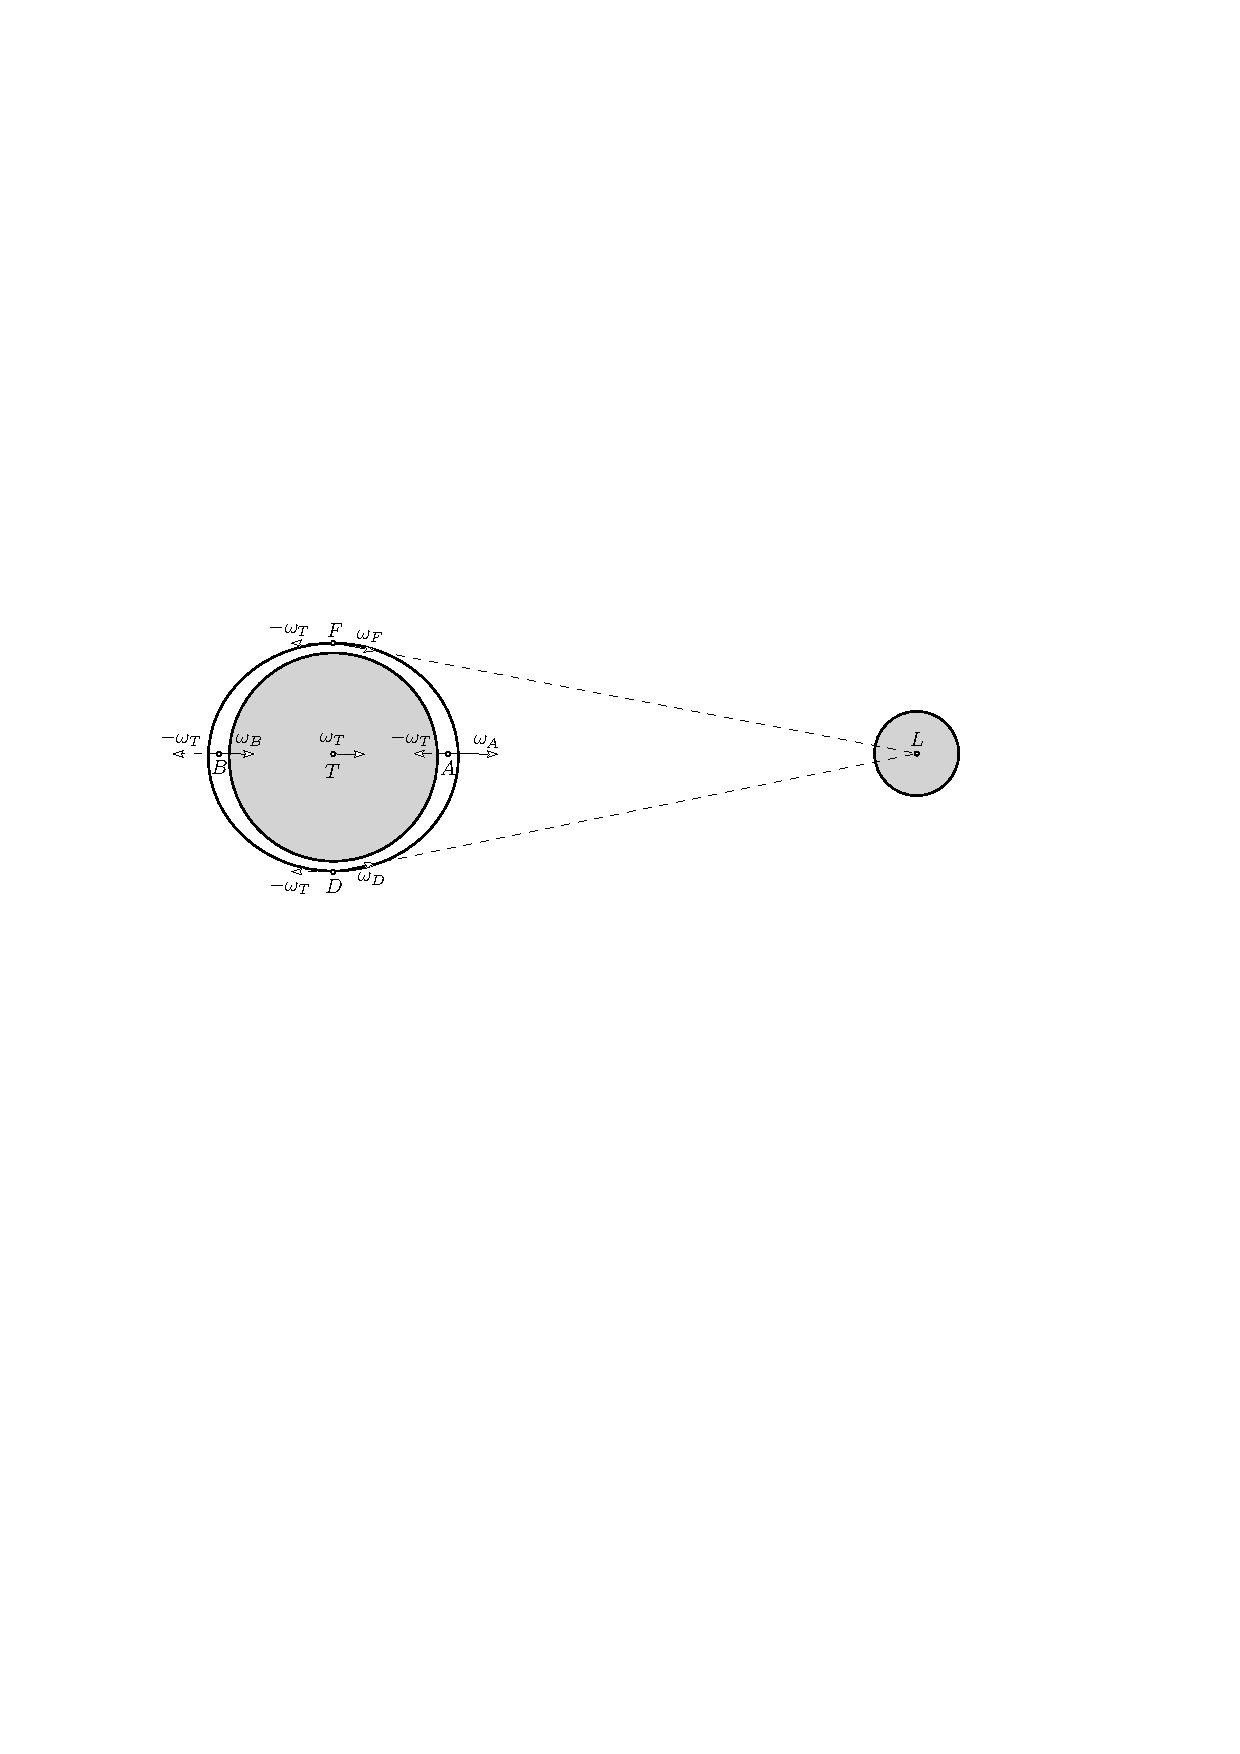
\includegraphics[width = 1\textwidth]{Ebb_flow}
\begin{figure}[h!]
\caption{К объяснению приливных сил}\label{Ebb_flow}
\end{figure}
\end{center}
